\section{Introduction}\label{S:introduction}

Cities worldwide continue to invest heavily in urban rail systems to connect residents to job centers \citep{uitp2024globalmetro}, yet whether these investments raise the incomes of the residents they serve remains an open question. Much of the existing evidence speaks instead to capitalization into property values: transit access raises housing prices near stations and along transport corridors \citep{diaz1999impacts, cohen2007impacts, wrigley2001transport, koutsopoulos1977impact, hess2007impact}. Whether this value reaches residents as real income growth---rather than being captured by landowners or dissipated through residential turnover---is far less settled: the estimated effect of transit proximity on local income ranges from positive to null to negative, depending on selection into treated areas and on how commuting and displacement are measured \citep{banerjee2020road, fogel1962quantitative, fogel1964railroads}.

Most of the empirical evidence on this question comes from advanced economies \citep{mohammad2013meta, gonzalez2018subways}, while mass transit is plausibly more consequential for income in developing-country cities, where the evidence base is thinner and commuting costs and uneven transit provision loom larger \citep{tsivanidis2026evaluating, storeygard2025transportLMIC, moreno2016access, iimi2019jobaccessibility}. In this context of developing-country cities, this paper turns to Brasília, Brazil's capital. Brasília's modernist core and central business district (CBD), the \textit{Plano Piloto}, is a purpose-built urban design with rigid land-use rules and limited housing capacity: much of the city's growth has been absorbed by satellite cities farther from the center, even as employment and public services remain highly concentrated in the core \citep{de2025evolution, unesco1987brasilia, acioly1992brasilia}. Because the \textit{Plano Piloto} is legally protected from densification, Brasília blocks the channel that \cite{glaeser2018economic} show usually connects workers to a city's income gains: where housing supply can expand, residents move closer to jobs and share in the income gains of the productive core. Where densification is blocked, as in Brasília, that option disappears: residents cannot move closer to jobs, and any income gains are instead capitalized into housing prices rather than reaching residents directly. Mass transit is a substitute for this blocked channel: workers cannot move closer to the center, but the subway can shorten their commute to it, so income gains are more likely to reach current residents directly rather than being captured only by whoever can afford to move in. Brasília therefore represents an extreme version of a situation common to many cities with expensive, supply-constrained centers: when moving closer to jobs is not an option, can transit still raise the incomes of the workers who stay?

In this context, this paper investigates whether the construction and operation of the Brasília Subway System increased income growth in areas exposed to the system, and, in particular, whether that growth reflects real income gains among the residents who already lived there rather than a shift in who lives there. To do so, we use IBGE census-tract data for Brasília in 2000, before the subway was implemented, and 2010, when the subway was already in operation, and use income growth over the decade as the main outcome. To perform this analysis, we use an instrumental-variables approach that leverages a planned and discarded subway alignment to address the potential endogeneity of station placement, controlling for baseline tract characteristics and administrative-region fixed effects. First, we estimate whether census tracts exposed to the subway experienced higher income growth between 2000 and 2010 than non-exposed tracts. Second, we subject these estimates to a battery of robustness checks that vary the geographic scope of the comparison group, the distance threshold used to define treatment, and the functional form of the exposure measure, assessing whether the main finding holds across alternative specification choices. Third, and crucially for the interpretation of the first set of results, we ask whether that income growth represents real gains for the residents who already lived in exposed tracts, by testing three hypotheses. Two rule out alternative explanations: that the effect reflects changes in the physical structure of exposed areas, or demographic sorting, meaning higher-income households replace lower-income incumbents. The third hypothesis adds a direct, positive argument for the same conclusion. Since job access itself cannot be measured directly, the labor-market hypothesis asks whether household-head income moved the way improved job access would predict: a larger share of household heads earning some income, and existing earners earning more.

Our results indicate that census tracts exposed to a subway station experienced income growth approximately 10 percent higher than otherwise comparable tracts over the 2000–2010 decade, a positive and statistically significant effect that is consistent across specifications with increasingly comprehensive sets of controls. This estimate holds across different specification tests: the point estimate remains positive and of similar magnitude when the geographic scope of the comparison group is varied, when the distance threshold used to define treatment is varied, and when the binary exposure indicator is replaced by continuous intensity-based measures of proximity. To assess whether this result reflects real income gains among incumbent residents, three mechanisms are tested. Two are alternative explanations: an urban structure hypothesis, under which income growth follows from subway-induced physical densification rather than from improved labor-market access; and a demographic composition hypothesis, under which tract-level income rises through the displacement of lower-income residents and their replacement by wealthier ones. Neither finds support in the data. Having ruled out both, the third hypothesis supplies a direct, positive argument for the same conclusion. Because job access cannot be measured directly, the labor-market hypothesis is tested by decomposing the income effect into an extensive margin---the share of household heads with positive income---and an intensive margin---the average income of those who already had it. Both margins respond positively and significantly to subway exposure, evidence that the income effect reflects real income gains among the residents already living in subway-exposed areas, consistent with the labor-market channel.

This paper is related to a literature asking whether mass transit raises local income, and more specifically, whether it raises the income of the residents who already lived there. Transport investments are thought to reshape a city's economic geography by changing how its residents interact with it---cheaper, faster connections change where people can realistically work relative to where they live \citep{duranton2012urban}. For mass transit specifically, a few studies find that it raises local income. \citet{heilmann2018transit}, exploiting a Dallas rail network that was extensively planned but only partially built, finds that census tracts that received light-rail access saw their median family income rise relative to tracts that were promised access but did not receive it. \citet{yen2024rapid}, instrumenting station placement in Los Angeles with a hypothetical least-cost Metro route, finds that residents living near new stations saw their earnings rise by as much as 26 percent. \citet{mayertrevien2017largescale} find a comparable employment gain, 12.8 percent, in municipalities connected to a new commuter-rail line in the Paris region. What none of these studies can settle is whose income rose.

In each case, the authors themselves attribute part or all of the gain to a change in who lives or works in the area rather than to income growth among incumbent residents. \citet{heilmann2018transit} attributes Dallas's income gain to housing turnover: poorer households move out as land near stations grows more valuable, wealthier ones move in, and the tract's income rises without any resident's income doing so. \citet{mayertrevien2017largescale} report the same pattern for Paris: population overall is unaffected, but the share of high-skill residents rises near new stations, which they interpret as ``a population displacement effect: a shift toward more wealthy residents around new stations'' rather than income growth for anyone already there. \citet{tyndall2021local} finds the same pattern across four U.S. metros: light rail stations raise neighborhood-level employment, but a structural neighborhood-choice model shows this operates by pricing low-skilled workers out of accessible areas and into more isolated ones, so that light rail transit lowers aggregate metropolitan employment even as it raises it locally. \citet{yen2024rapid} reaches a related but distinct conclusion: earnings near new Los Angeles stations rise most where local job density also rises, suggesting the gain reflects new economic activity moving into the area rather than existing residents reaching jobs they could not reach before. A credible claim that a subway raised the incomes of its existing residents has to rule out both of these stories---compositional change and physical or economic restructuring of the area---not merely report a positive coefficient on tract income. This is a demanding standard, and one that developing-country cities have not yet been held to: the evidence above comes entirely from cities in the United States and France, while commuting costs and the returns to closing a job-access gap are plausibly larger where transit provision is thinner and more uneven \citep{tsivanidis2026evaluating}.

This paper is built to close that gap, contributing to the literature on mass transit and urban economic outcomes in three ways. First, it provides causal evidence on the income effects of subway exposure in a developing-country context, where commuting frictions, labor-market structure, and spatial inequality differ substantially from the settings that dominate the empirical literature, and where the welfare consequences of transit investment may therefore be qualitatively different. Second, the paper contributes methodologically by exploiting a planned and subsequently discarded subway alignment as an instrument for realized station proximity, and by conducting the analysis at the fine-grained census-tract level. Third, unlike \citet{heilmann2018transit}, \citet{mayertrevien2017largescale}, and \citet{tyndall2021local}, who attribute comparable local gains to a change in who lives or works in the exposed area, this paper shows that the income gains documented here are accompanied by neither: they reflect real income growth among the residents who already lived in exposed tracts, closing the gap left open above.

The present paper is structured as follows. Section~\ref{s:subway} describes the Brasília subway system, its history, spatial configuration, and the planned and discarded alignment used as the instrument. Section~\ref{s:data} describes the census-tract data, the construction of the exposure and instrument measures, and presents descriptive statistics. Section~\ref{s:methodology} presents the empirical strategy, detailing the 2SLS approach, the construction of the exposure and instrument variables, and the role of administrative-region fixed effects. Section~\ref{s:results} presents the main estimates and a series of robustness tests that vary the geographic scope of the comparison group, the distance threshold used to define treatment, and the functional form of the exposure measure. Section~\ref{s:mechanisms} investigates the mechanisms behind the estimated income effect, ruling out urban structure changes and demographic composition shifts in subway-exposed areas before testing the labor-market channel directly. Finally, Section~\ref{s:conclusion} presents the paper's conclusions.

\section{The Brasília Subway System}\label{s:subway}

Proposals for a rail-based transit system in the Federal District predate its construction by more than two decades. A preliminary plan was presented to the local government in 1976 but was judged unfeasible. A formal feasibility study was subsequently commissioned from the Mauá Institute of Technology (\textit{Instituto Mauá de Tecnologia}, IMT) in 1986--1987, which produced a network design that was set aside in favor of further studies; the project eventually built corresponded to a later design, contracted under a subsequent administration. Construction began in 1992 but was marked by repeated interruptions driven by hyperinflation and contested federal transfers. Commercial service started only in September 2001, more than seven years after the original target date, and the network was subsequently expanded over the following two decades.

In its current configuration, the system comprises two operating lines---the Green Line and the Orange Line---totaling 27 stations across 42 km of track \citep{institutomdt2019evolucao}. The two lines run from Central station, in the \textit{Plano Piloto}, and bifurcate toward Ceilândia and Samambaia via Taguatinga, serving six administrative regions in total. Because of the long distances between many stations and the low residential densities along the corridor, the system functions largely as an inter-regional connector rather than as a fine-grained intra-urban network. Figure~\ref{fig:subway_system} maps the network and names the six administrative regions it serves, making explicit the corridor running from Central station, in the \textit{Plano Piloto}, westward to Ceilândia and Samambaia.

\begin{figure}[h!]
\caption{The Brasília Subway System and the Administrative Regions It Serves}
\label{fig:subway_system}
\centering
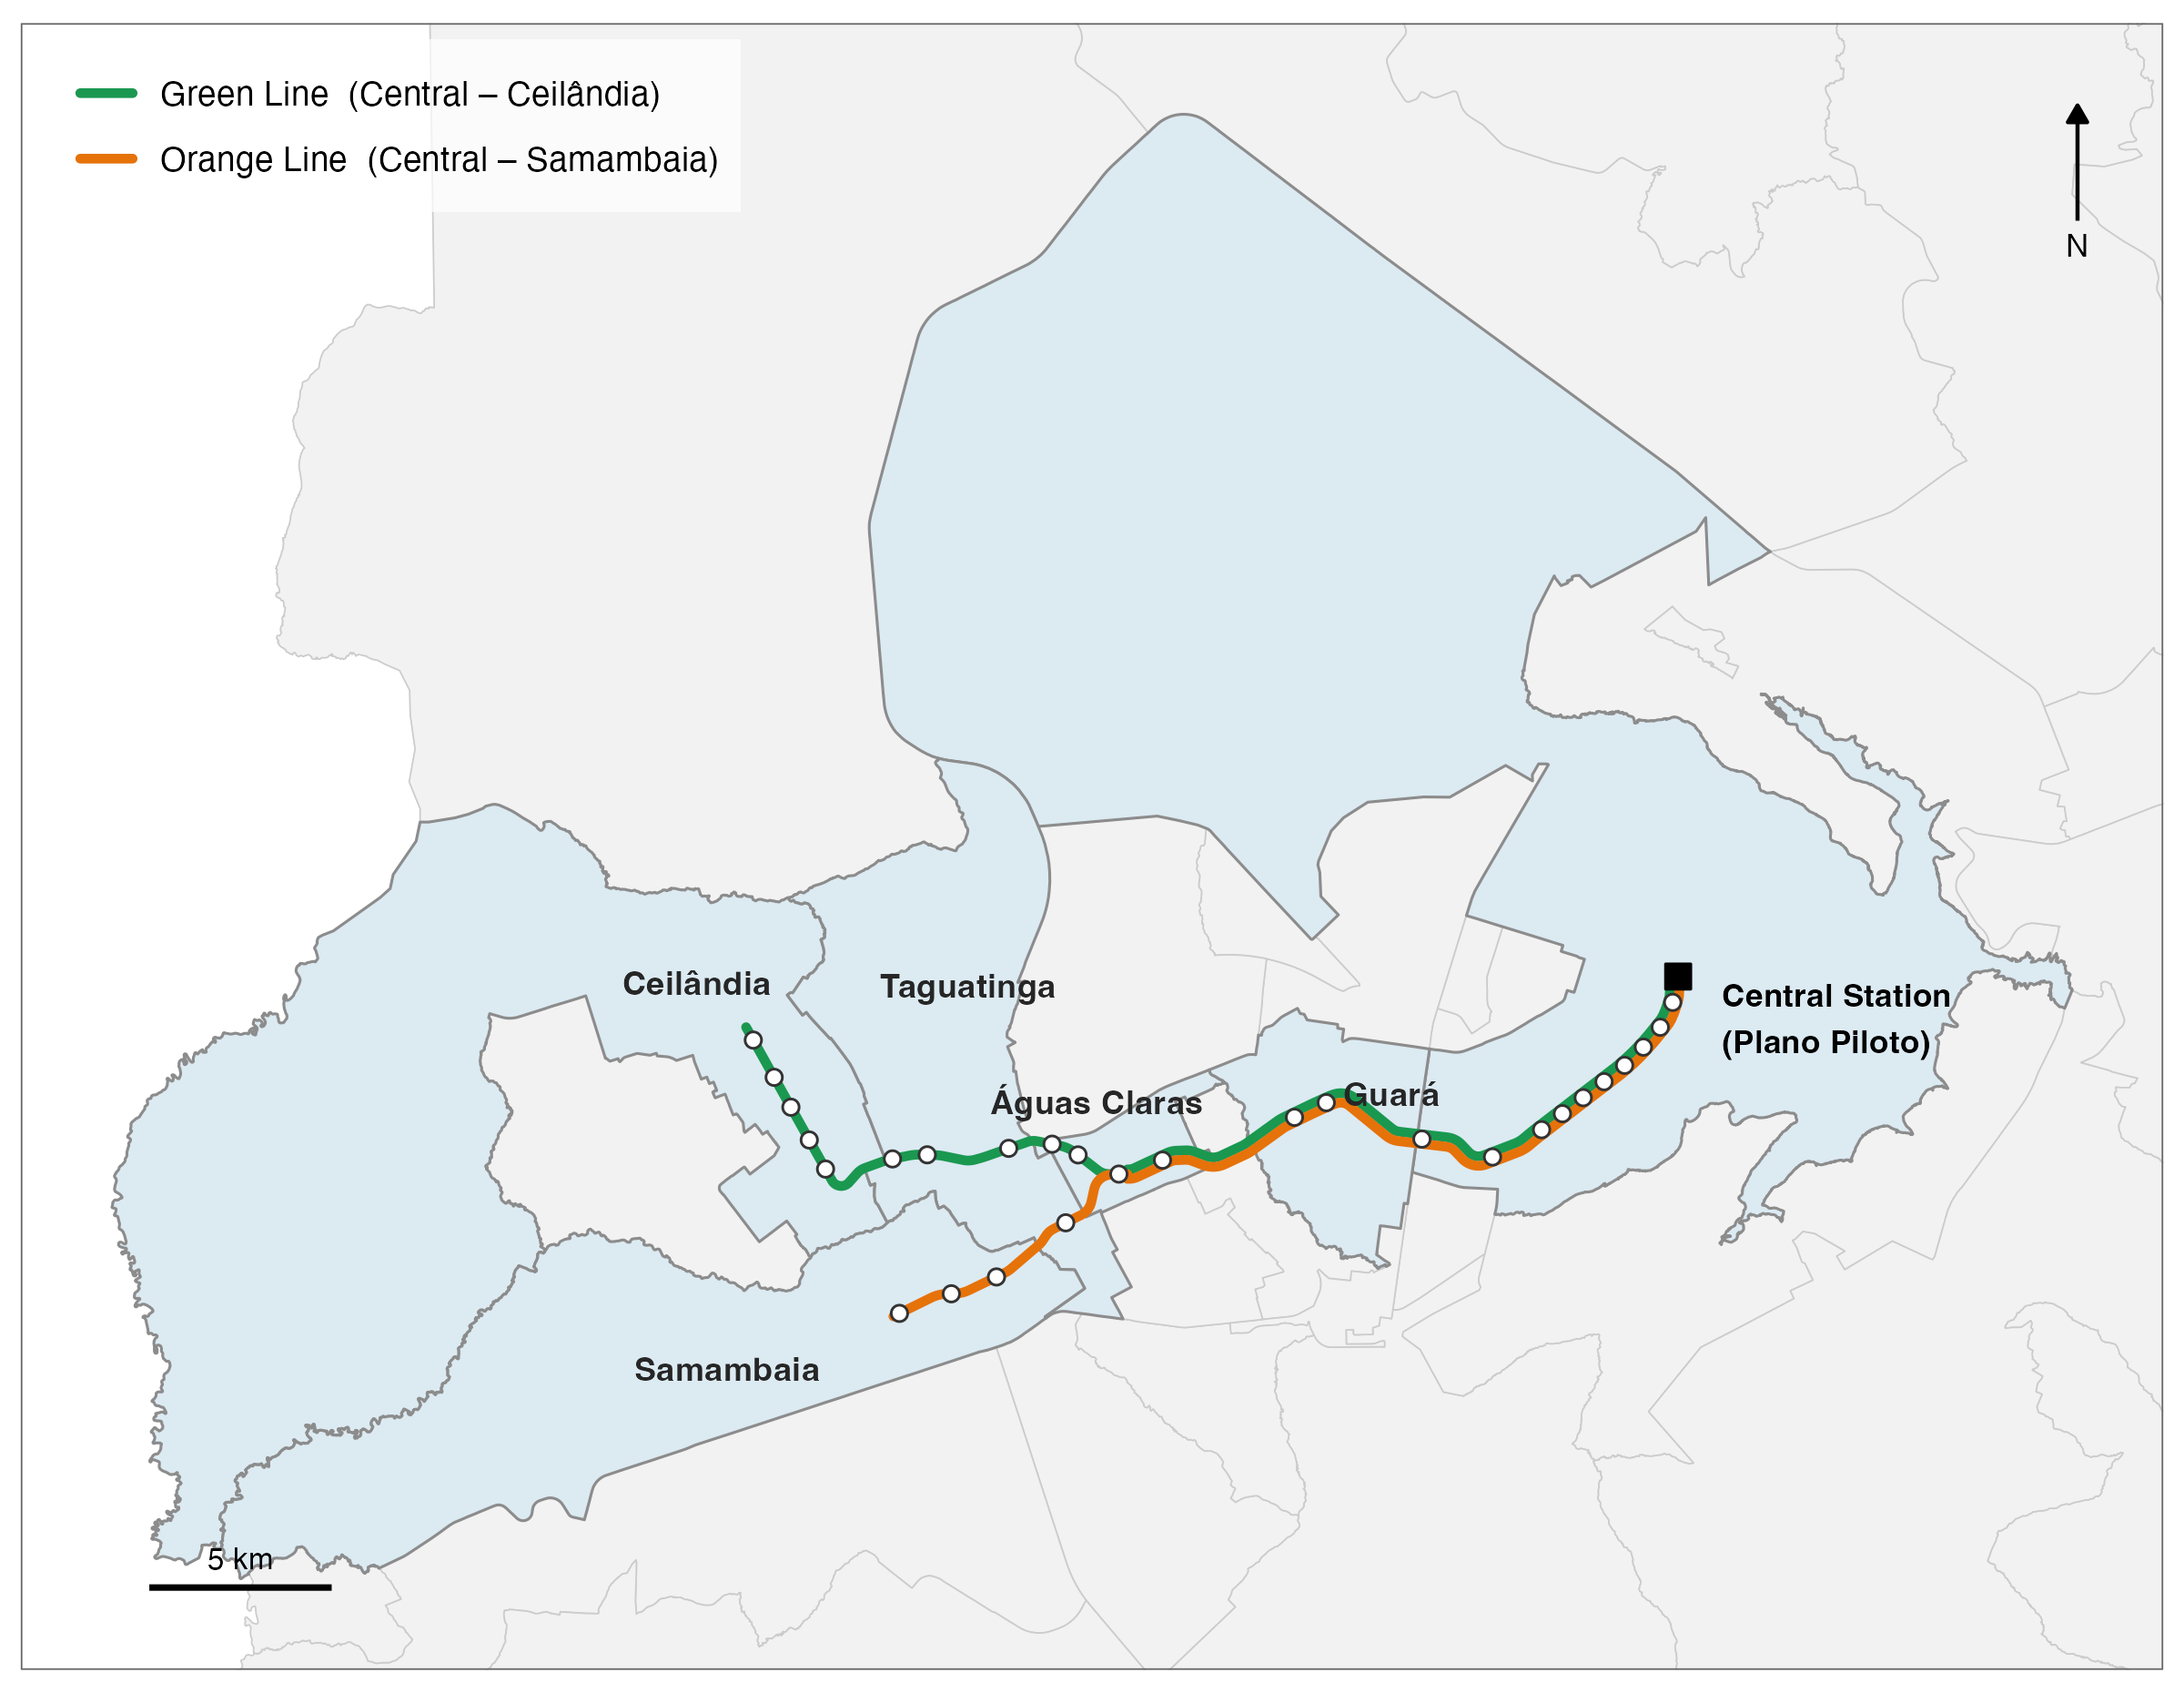
\includegraphics[width=0.92\textwidth]{images/subway_system_bsb.png}
\vspace{-0.2cm}
\begin{flushleft}
\footnotesize \textit{Note}: The map shows the two operating lines of the Brasília subway system, their stations, and the six administrative regions (RAs) served by the network, identified by name. The Green Line links Central station---located at the \textit{Plano Piloto} bus terminal, in Brasília's employment core---to Ceilândia, and the Orange Line branches toward Samambaia; both lines share the central trunk and bifurcate near Taguatinga. Highlighted polygons indicate the served RAs; remaining RAs of the Federal District are shown in grey for context. Coordinates are in SIRGAS 2000 / UTM zone 23S. \textit{Source}: Brasília GeoPortal (GeoPortal/DF); authors' elaboration.
\end{flushleft}
\end{figure}

This spatial configuration is precisely what makes the system relevant to the question studied in this paper. Brasília's employment and public services remain heavily concentrated in the legally protected \textit{Plano Piloto}, while most of the population resides in distant satellite cities, a separation between residence and workplace that is actively maintained by the city's land-use regime \citep{de2025evolution}.\footnote{See also \citep{codeplan2018expansao} on the socioeconomic profile of the subway's direct area of influence.} By connecting lower-income peripheral regions such as Ceilândia, Samambaia, and Taguatinga to the central labor market, the subway would operate as a labor-market access shock for the residents of exposed areas. The scale of this connection is non-trivial: the system carried approximately 42.5 million passengers in 2024, an average of about 3.5 million per month and on the order of 148,000 passengers on a typical weekday, with Central station, at the \textit{Plano Piloto} bus terminal, by far the busiest node in the network.\footnote{Ridership figures are reported in the \href{https://agenciabrasilia.df.gov.br/w/metro-df-passa-dos-425-milhoes-de-passageiros-ao-ano-e-projeta-ampliacao-para-2025/}{Metrô-DF Annual Administration Report for 2024} and in associated official communications of the Federal District government.}

For the purposes of identification, the most relevant feature of this history is the existence of a planned but unbuilt alignment. The 1986--1987 IMT feasibility study produced a network design that was set aside in favor of subsequent studies and was never implemented. The historical record does not provide a public, definitive explanation for why the IMT proposal was discarded. Several factors plausibly contributed and are consistent with the documented sequence of events: the change of state administration between the design's completion and the eventual construction phase; the financing difficulties that surrounded the project throughout the late 1980s and early 1990s; and a technical reassessment of the system's design, including its mode and alignment. The available evidence suggests that the abandonment reflected the institutional and political circumstances of the period rather than the income trajectories of individual census tracts---an assumption that is central to the instrumental-variable strategy developed in Section~\ref{s:methodology}, which uses proximity to this discarded alignment as an instrument for realized subway exposure.